%% LyX 2.4.4 created this file.  For more info, see https://www.lyx.org/.
%% Do not edit unless you really know what you are doing.
\documentclass[english]{article}
\usepackage[T1]{fontenc}
\usepackage[latin9]{inputenc}
\usepackage{cancel}

\makeatletter
%%%%%%%%%%%%%%%%%%%%%%%%%%%%%% User specified LaTeX commands.
\usepackage{hyperref}
\usepackage[usenames,dvipsnames,table]{xcolor} %adds additional color options
\hypersetup{colorlinks=true, urlcolor=black,linkcolor=black}

\usepackage{fancyhdr}
\usepackage{lastpage}
\pagestyle{fancy}
\usepackage{enumitem}
\usepackage{ifthen}
%sets math fonts to be more readable
%\everymath=\expandafter{\the\everymath\displaystyle}
%\DeclareMathSizes{10}{10}{10}{10}
\usepackage{multicol}

\usepackage{tikz}
\usetikzlibrary{plotmarks}
\usepackage{pgfplots}
\pgfplotsset{compat=newest}

\usepackage{calc}
\usepackage[nomessages]{fp}

\usepackage{advdate}    % Advancing/saving dates
\usepackage{datetime}   % Dates formatting
\usepackage{datenumber} % Counters for dates

\usepackage{fancybox} %%ovalbox and fancy box settings

\usepackage[super]{nth} %easy 1st, 2nd, etc

\usepackage{forest} %%for tree diagram

%%data for histogram%%
\begin{filecontents}{hist1_data.csv} 
dist 
3
1
0
4
1
3
2
2
0
2
0
2
2
1
4
3
1
1
3
4
2
1
3
0
1
0
2
5
1
2
3
0
0
1
2
3
1
2
0
2
\end{filecontents}

%%data for histogra: cal per cereal%%
\begin{filecontents}{hist_data_cereal.csv} 
dist 
3.7
3.6
3.6
4.0
4.0
3.6
3.8
3.7
4.1
3.9
3.9
3.3
3.5
3.6
3.9
4.0
\end{filecontents}

\makeatother

\usepackage{babel}
\begin{document}
\newcommand{\gauss}[2]{1/(#2*sqrt(2*pi))*exp(-((x-#1)^2)/(2*#2^2))}

\newcommand{\normalcdf}[4]{ %mean,std,z-left,z-right
\begin{tikzpicture}[scale=1.25]

\pgfmathsetmacro{\mn}{#1}
\pgfmathsetmacro{\sd}{#2}
\pgfmathsetmacro{\za}{#1+#2*1}
\pgfmathsetmacro{\zb}{#1+#2*2}
\pgfmathsetmacro{\zc}{#1+#2*3}

\pgfmathsetmacro{\zna}{#1-#2*1}
\pgfmathsetmacro{\znb}{#1-#2*2}
\pgfmathsetmacro{\znc}{#1-#2*3}

\pgfmathsetmacro{\zleft}{#3}
\pgfmathsetmacro{\zright}{#4}
\pgfmathsetmacro{\zsL}{(#3-#1)/#2} %z-score
\pgfmathsetmacro{\zsR}{(#4-#1)/#2} %z-score
\pgfmathsetmacro{\xCenter}{\zsL/2.5+\zsR/2.5} %center using z-score
\pgfmathsetmacro{\yCenter}{((1/(1*sqrt(2*pi))*exp(-((\xCenter-0)^2)/(2*1^2)))/2}
\pgfkeys{/pgf/fpu} %for large numbers
\pgfmathparse{100*(1/(1 + exp(-0.07056*((\zsR-0)/1)^3 - 1.5976*(\zsR-0)/1))-1/(1 + exp(-0.07056*((\zsL-0)/1)^3 - 1.5976*(\zsL-0)/1)))} %area from z-left to z-right
\edef\area{\pgfmathresult} 
\pgfkeys{/pgf/fpu=false}

\scriptsize
\begin{axis}[ 
	no markers, 
	domain=0:10, 
	%samples=100, 
	axis lines*=left, 
	%xlabel=Standard deviations, 
	%ylabel=Frequency, 
	height=2.5cm, %change/remove this scaling to get 1:1 pic
	width=5.5cm, 
	hide y axis,
	%ticks=none,
	xtick={-3,-2,-1,0,1,2,3},
	xticklabels={\pgfmathprintnumber[precision=0]{\znc},\pgfmathprintnumber[precision=2]{\znb},\pgfmathprintnumber[precision=2]{\zna},#1,\pgfmathprintnumber[precision=0]{\za},\pgfmathprintnumber[precision=2]{\zb},\pgfmathprintnumber[precision=2]{\zc}},
	%xticklabels={-25, -15, -5, 5, 15, 25, 35},
	%ytick=empty, 
	enlargelimits=false, 
	clip=false, 
	axis on top, 
	%grid = major
	]

	\addplot [fill=blue!35, draw=red,  domain=\zsL:\zsR] {\gauss{0}{1}} \closedcycle;
		\node (arrowEnd) at (axis cs: \xCenter, \yCenter) {};
	\addplot [draw, thick, smooth, domain=-3:3] {\gauss{0}{1}} \closedcycle;
		\node[anchor=south east] (arrowStart) at (current bounding box.east) {\pgfmathprintnumber[fixed,precision=1]{\area}\%};
	\draw[->,thick,black] (arrowStart) to (arrowEnd);
	
	%\addplot [fill=orange!20, draw=none, domain=2:3] {\gauss{0}{1}} \closedcycle; 
	%\addplot [fill=blue!20, draw=none, domain=-2:-1] {\gauss{0}{1}} \closedcycle; 
	%\addplot [fill=blue!20, draw=none, domain=1:2] {\gauss{0}{1}} \closedcycle; 
	%\only<1->{\node[above] at (axis cs: -0.5, 0.025) {$34.1\%$};} 
	%\only<1->{\node[above] at (axis cs: 0.5, 0.025) {$34.1\%$};} 
	%\only<1->{\node[above] at (axis cs: -1.5, 0.025) {$13.6\%$};}
	%\only<1->{\node[above] at (axis cs: 1.5, 0.025) {$13.6\%$};}
	%\only<1->{\node[above] at (axis cs: 2.5, 0.05) {$2.1\%$};}
	%\only<1->{\node[above] at (axis cs: -2.5, 0.05) {$2.1\%$};}
	%\only<1->{ \addplot[<->,black,very thick] coordinates {(-1,0.4) (1,0.4)};} 
	%\only<1->{\node[above] at (axis cs: 0, 0.4) {$68.2\%$};} 
	%\only<1->{\addplot[<->,black,very thick] coordinates {(-2,0.3) (2,0.3)};}
	%\only<1->{\node[above] at (axis cs: 0, 0.3) {$95.4\%$};}
	%\only<1->{\addplot[<->,black, very thick] coordinates {(-3,0.2) (3,0.2)};} 
	%\only<1->{\node[above] at (axis cs: 0, 0.2) {$99.7\%$};}
	\end{axis} 
\end{tikzpicture}
}

\newcommand{\normalpdf}[5]{ %mean,std,z-left,z-right
\begin{tikzpicture}[scale=1.25]

\pgfmathsetmacro{\mn}{#1}
\pgfmathsetmacro{\sd}{#2}
\pgfmathsetmacro{\za}{#1+#2*1}
\pgfmathsetmacro{\zb}{#1+#2*2}
\pgfmathsetmacro{\zc}{#1+#2*3}

\pgfmathsetmacro{\zna}{#1-#2*1}
\pgfmathsetmacro{\znb}{#1-#2*2}
\pgfmathsetmacro{\znc}{#1-#2*3}

\pgfmathsetmacro{\zleft}{#3}
\pgfmathsetmacro{\zright}{#4}
\pgfmathsetmacro{\zsL}{(#3-#1)/#2} %z-score
\pgfmathsetmacro{\zsR}{(#4-#1)/#2} %z-score
\pgfmathsetmacro{\zsV}{(#5-#1)/#2} %z-score
\pgfmathsetmacro{\xCenter}{\zsL/2.5+\zsR/2.5} %center using z-score
\pgfmathsetmacro{\yCenter}{((1/(1*sqrt(2*pi))*exp(-((\xCenter-0)^2)/(2*1^2)))/2}
\pgfkeys{/pgf/fpu} %for large numbers
\pgfmathparse{100*(1/(1 + exp(-0.07056*((\zsR-0)/1)^3 - 1.5976*(\zsR-0)/1))-1/(1 + exp(-0.07056*((\zsL-0)/1)^3 - 1.5976*(\zsL-0)/1)))} %area from z-left to z-right
\edef\area{\pgfmathresult} 
\pgfkeys{/pgf/fpu=false}

\scriptsize
\begin{axis}[ 
	no markers, 
	domain=0:10, 
	%samples=100, 
	axis lines*=left, 
	%xlabel=Standard deviations, 
	%ylabel=Frequency, 
	height=2.5cm, %change/remove this scaling to get 1:1 pic
	width=5.5cm, 
	hide y axis,
	%ticks=none,
	xtick={\zsV},
	xticklabels={\pgfmathprintnumber[precision=2]{#5}},
	%xticklabels={-25, -15, -5, 5, 15, 25, 35},
	%ytick=empty, 
	enlargelimits=false, 
	clip=false, 
	axis on top, 
	%grid = major
	]

	\addplot [fill=blue!35, draw=red,  domain=\zsL:\zsR] {\gauss{0}{1}} \closedcycle;
		\node (arrowEnd) at (axis cs: \xCenter, \yCenter) {};
	\addplot [draw, thick, smooth, domain=-3:3] {\gauss{0}{1}} \closedcycle;
		\node[anchor=south east] (arrowStart) at (current bounding box.east) {\pgfmathprintnumber[fixed,precision=1]{\area}\%};
	\draw[->,thick,black] (arrowStart) to (arrowEnd);
	
	%\addplot [fill=orange!20, draw=none, domain=2:3] {\gauss{0}{1}} \closedcycle; 
	%\addplot [fill=blue!20, draw=none, domain=-2:-1] {\gauss{0}{1}} \closedcycle; 
	%\addplot [fill=blue!20, draw=none, domain=1:2] {\gauss{0}{1}} \closedcycle; 
	%\only<1->{\node[above] at (axis cs: -0.5, 0.025) {$34.1\%$};} 
	%\only<1->{\node[above] at (axis cs: 0.5, 0.025) {$34.1\%$};} 
	%\only<1->{\node[above] at (axis cs: -1.5, 0.025) {$13.6\%$};}
	%\only<1->{\node[above] at (axis cs: 1.5, 0.025) {$13.6\%$};}
	%\only<1->{\node[above] at (axis cs: 2.5, 0.05) {$2.1\%$};}
	%\only<1->{\node[above] at (axis cs: -2.5, 0.05) {$2.1\%$};}
	%\only<1->{ \addplot[<->,black,very thick] coordinates {(-1,0.4) (1,0.4)};} 
	%\only<1->{\node[above] at (axis cs: 0, 0.4) {$68.2\%$};} 
	%\only<1->{\addplot[<->,black,very thick] coordinates {(-2,0.3) (2,0.3)};}
	%\only<1->{\node[above] at (axis cs: 0, 0.3) {$95.4\%$};}
	%\only<1->{\addplot[<->,black, very thick] coordinates {(-3,0.2) (3,0.2)};} 
	%\only<1->{\node[above] at (axis cs: 0, 0.2) {$99.7\%$};}
	\end{axis} 
\end{tikzpicture}
}

\newcommand{\normalpdfB}[4]{ %mean,std,z-left,z-right
\begin{tikzpicture}[scale=1.25]

\pgfmathsetmacro{\mn}{#1}
\pgfmathsetmacro{\sd}{#2}
\pgfmathsetmacro{\za}{#1+#2*1}
\pgfmathsetmacro{\zb}{#1+#2*2}
\pgfmathsetmacro{\zc}{#1+#2*3}

\pgfmathsetmacro{\zna}{#1-#2*1}
\pgfmathsetmacro{\znb}{#1-#2*2}
\pgfmathsetmacro{\znc}{#1-#2*3}

\pgfmathsetmacro{\zleft}{#3}
\pgfmathsetmacro{\zright}{#4}
\pgfmathsetmacro{\zsL}{(#3-#1)/#2} %z-score
\pgfmathsetmacro{\zsR}{(#4-#1)/#2} %z-score
\pgfmathsetmacro{\xCenter}{\zsL/2.5+\zsR/2.5} %center using z-score
\pgfmathsetmacro{\yCenter}{((1/(1*sqrt(2*pi))*exp(-((\xCenter-0)^2)/(2*1^2)))/2}
\pgfkeys{/pgf/fpu} %for large numbers
\pgfmathparse{100*(1/(1 + exp(-0.07056*((\zsR-0)/1)^3 - 1.5976*(\zsR-0)/1))-1/(1 + exp(-0.07056*((\zsL-0)/1)^3 - 1.5976*(\zsL-0)/1)))} %area from z-left to z-right
\edef\area{\pgfmathresult} 
\pgfkeys{/pgf/fpu=false}

\scriptsize
\begin{axis}[ 
	no markers, 
	domain=0:10, 
	%samples=100, 
	axis lines*=left, 
	%xlabel=Standard deviations, 
	%ylabel=Frequency, 
	height=2.5cm, %change/remove this scaling to get 1:1 pic
	width=5.5cm, 
	hide y axis,
	%ticks=none,
	xtick={\zsL,\zsR},
	xticklabels={\pgfmathprintnumber[precision=2]{\zsL},\pgfmathprintnumber[precision=2]{\zsR}},
	%xticklabels={-25, -15, -5, 5, 15, 25, 35},
	%ytick=empty, 
	enlargelimits=false, 
	clip=false, 
	axis on top, 
	%grid = major
	]

	\addplot [fill=blue!35, draw=red,  domain=\zsL:\zsR] {\gauss{0}{1}} \closedcycle;
		\node (arrowEnd) at (axis cs: \xCenter, \yCenter) {};
	\addplot [draw, thick, smooth, domain=-3:3] {\gauss{0}{1}} \closedcycle;
		\node[anchor=south east] (arrowStart) at (current bounding box.east) {\pgfmathprintnumber[fixed,precision=1]{\area}\%};
	\draw[->,thick,black] (arrowStart) to (arrowEnd);
	
	%\addplot [fill=orange!20, draw=none, domain=2:3] {\gauss{0}{1}} \closedcycle; 
	%\addplot [fill=blue!20, draw=none, domain=-2:-1] {\gauss{0}{1}} \closedcycle; 
	%\addplot [fill=blue!20, draw=none, domain=1:2] {\gauss{0}{1}} \closedcycle; 
	%\only<1->{\node[above] at (axis cs: -0.5, 0.025) {$34.1\%$};} 
	%\only<1->{\node[above] at (axis cs: 0.5, 0.025) {$34.1\%$};} 
	%\only<1->{\node[above] at (axis cs: -1.5, 0.025) {$13.6\%$};}
	%\only<1->{\node[above] at (axis cs: 1.5, 0.025) {$13.6\%$};}
	%\only<1->{\node[above] at (axis cs: 2.5, 0.05) {$2.1\%$};}
	%\only<1->{\node[above] at (axis cs: -2.5, 0.05) {$2.1\%$};}
	%\only<1->{ \addplot[<->,black,very thick] coordinates {(-1,0.4) (1,0.4)};} 
	%\only<1->{\node[above] at (axis cs: 0, 0.4) {$68.2\%$};} 
	%\only<1->{\addplot[<->,black,very thick] coordinates {(-2,0.3) (2,0.3)};}
	%\only<1->{\node[above] at (axis cs: 0, 0.3) {$95.4\%$};}
	%\only<1->{\addplot[<->,black, very thick] coordinates {(-3,0.2) (3,0.2)};} 
	%\only<1->{\node[above] at (axis cs: 0, 0.2) {$99.7\%$};}
	\end{axis} 
\end{tikzpicture}
}

From file

\begin{tikzpicture}[scale=.75]
\begin{axis}[     ybar,     ymin=0 ]
\addplot+[hist={bins=10}] table [y index=0] {men_height.csv};
\end{axis} 
\end{tikzpicture} 

From preamble data

\begin{tikzpicture}[scale=.8]
\begin{axis}[     ybar,     ymin=0 ] 
\addplot +[hist={bins=5,data min=3.2,data max=4.2}] table [y index=0] {hist_data_cereal.csv}; 
\end{axis} 
\end{tikzpicture} 

From frequency table

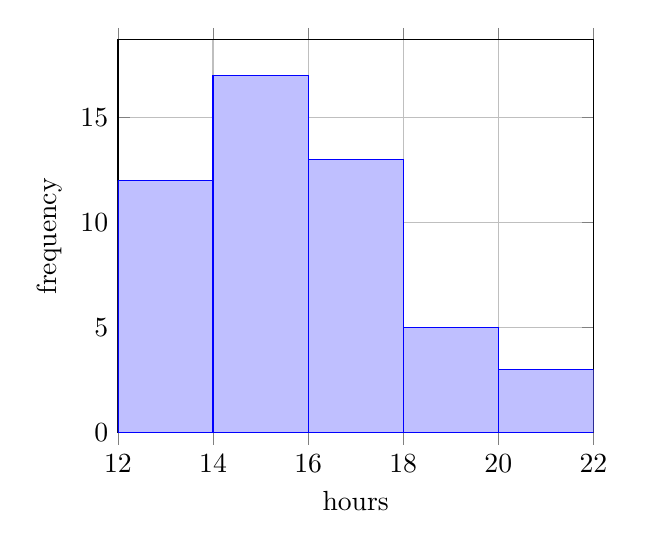
\begin{tikzpicture}[scale=1]
\begin{axis}[     
	ybar interval,
	x tick label as interval=false,    
	ymin=0,
	xmin=12,
	xmax=22,
	width=3in,
	%height=3in,
	grid=major,
	ylabel=frequency,
	xlabel=hours
	] 
	\addplot [fill=blue!25,draw=blue] table [x=Lower, y=Count] { 
		Lower Upper Count 
		12	14	12
		14	16	17
		16	18	13
		18	20	5
		20	22	3
		22	24	0
	};
\end{axis}
\end{tikzpicture}
\end{document}
